\section{Fourier and the Decomposition of Motion: From Structure to Spectrum}

\subsection{The Equation That Shook Mathematics: Fourier and the Waves Beneath Everything}

If Cayley showed that geometry could be encoded in algebra,  
then Joseph Fourier revealed that motion itself could be decomposed into waves.

Where Cayley sought invariants under transformation,  
Fourier sought the elemental vibrations beneath complexity.

While Jacobi and Hamilton described mechanics in terms of flows and surfaces,  
and Cayley abstracted geometry into matrices and transformations,  
Fourier offered a different insight:

\begin{quote}
“What if the complexity of motion wasn’t complexity at all—  
but the superposition of simpler, sinusoidal modes?”
\end{quote}

Cayley’s matrices described how spaces could be transformed: stretched, rotated, projected.  
But Fourier introduced a way to transform functions themselves—  
to translate signals, motions, and even heat distributions into a new language.

Instead of describing a function \( f(x) \) directly,  express it as an infinite sum of sine and cosine functions:

\[
f(x) = \sum_{n=1}^{\infty} \left( a_n \cos(nx) + b_n \sin(nx) \right)
\]

Each coefficient \( a_n, b_n \) captured how much of a particular frequency was “inside” the original function.

At the heart of his method was what is now called a \textbf{Fourier series}. It was a way to express a function as an infinite sum of trigonometric functions:

\[
f(x) = a_0 + \sum_{n=1}^{\infty} \left( a_n \cos(n x) + b_n \sin(n x) \right).
\]

\begin{figure}[H]

\begin{center}
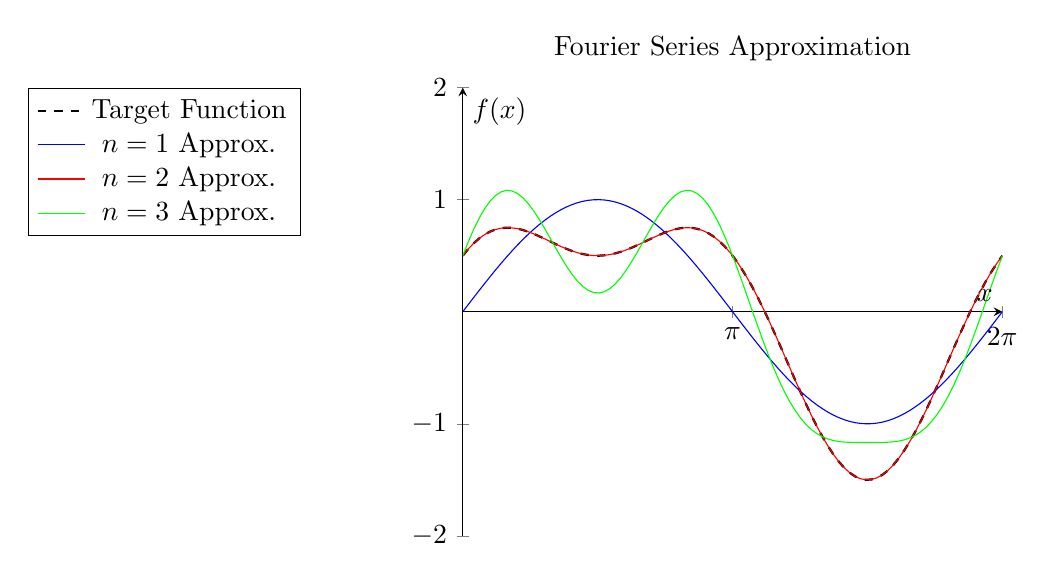
\begin{tikzpicture}
    \begin{axis}[
        domain=0:2*pi,
        samples=100,
        axis x line=middle,
        axis y line=middle,
        ymin=-2, ymax=2,
        xlabel={$x$}, ylabel={$f(x)$},
        xtick={0, 3.14, 6.28},
        xticklabels={$0$, $\pi$, $2\pi$},
        title={Fourier Series Approximation},
        legend style={at={(-0.3,1)}, anchor=north east} % Moves legend to the far left
    ]

        % Base function (target function)
        \addplot[thick, black, dashed, domain=0:2*pi] {sin(deg(x)) + cos(deg(2*x))/2};
        
        % First approximation (n=1)
        \addplot[blue, domain=0:2*pi] {sin(deg(x))};
        
        % Second approximation (n=2)
        \addplot[red, domain=0:2*pi] {sin(deg(x)) + cos(deg(2*x))/2};
        
        % Third approximation (n=3)
        \addplot[green, domain=0:2*pi] {sin(deg(x)) + cos(deg(2*x))/2 + sin(deg(3*x))/3};

        \legend{Target Function, $n=1$ Approx., $n=2$ Approx., $n=3$ Approx.}

    \end{axis}
\end{tikzpicture}
\end{center}
  \caption{PUT SOMETHING HERE}
\end{figure}


This equation says something remarkable: no matter how messy or irregular a function might seem, it could be reconstructed entirely from smooth waves. Fourier discovered that even functions describing complex heat distributions could be rewritten in this way, making it much easier to analyze how temperature evolved over time.

\begin{tcolorbox}[colback=gray!5!white, colframe=black, title=\textbf{Sidebar: The Shift from Cayley to Fourier}, fonttitle=\bfseries, arc=1.5mm, boxrule=0.4pt]

\begin{tabular}{>{\raggedright}p{4cm} >{\raggedright}p{5.5cm} >{\raggedright\arraybackslash}p{5.5cm}}
 & \textbf{Cayley} & \textbf{Fourier} \\
\midrule
Key object & Matrix as a transformation & Function as a sum of waves \\
View of complexity & Transformation between spaces & Decomposition into frequencies \\
Core operation & Matrix multiplication, determinant & Inner product with sine/cosine basis
\end{tabular}

\end{tcolorbox}


\subsection{A Language for Change: From Leibniz to Partial Differential Equations}

Fourier studied the classic PDE \textbf{heat equation}:

\[
\frac{\partial u}{\partial t} = \alpha \frac{\partial^2 u}{\partial x^2}
\]

Where:
\begin{itemize}
  \item \( u(x, t) \) is the temperature at position \( x \) and time \( t \),
  \item \( \alpha \) is the thermal diffusivity constant.
\end{itemize}

This equation tells us:  
\begin{itemize}
  \item how the temperature changes over time (\( \frac{\partial u}{\partial t} \))  
  \item depends on how curved or uneven the temperature is across space (\( \frac{\partial^2 u}{\partial x^2} \)).  
\end{itemize}

Solving this equation means figuring out how temperature behaves everywhere and at every moment, given how it spreads and smooths out.

\begin{quote}
\textit{Leibniz gave us the grammar to describe change; Fourier used it to write the dynamics of heat, sound, and waves themselves.}
\end{quote}

In the sections that follow, we’ll see how different partial differential equations capture two fundamental aspects of physical systems: how they evolve \emph{in time}, and how they are structured \emph{across space}.



\subsection{d’Alembert and the Wave Equation: Time in Motion}

In the mid-1700s, Jean le Rond d’Alembert studied the motion of vibrating strings and derived one of the earliest examples of what we now call a \textit{partial differential equation}: the wave equation.

In physical terms, a wave is any quantity that oscillates (i.e. it goes up and down over space or time), and they wave have these key features:

\begin{itemize}
  \item \textbf{Amplitude}: how tall the wave is — its maximum height from the center line.
  \item \textbf{Wavelength}: the horizontal distance over which the wave pattern repeats.
  \item \textbf{Frequency}: how many complete waves fit within a certain interval.
  \item \textbf{Phase}: the relative horizontal shift of a wave — it tells you where the wave starts in its cycle.
\end{itemize}

Sine waves are one of the simplest types, and they form the basic ingredients of more complex signals. It is an example of \textbf{trigonometric functions}, and they describe smooth, repeating wave patterns.

\begin{figure}[H]
  \centering

  % First row: Amplitude (left) and Wavelength (right)
  \begin{subfigure}[t]{0.45\textwidth}
    \centering
    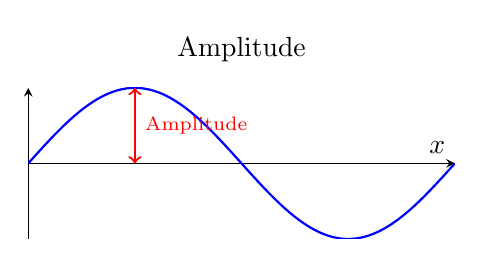
\begin{tikzpicture}
      \begin{axis}[
        axis lines = middle,
        xlabel = $x$,
        xtick=\empty,
        ytick=\empty,
        width=7cm,
        height=3.5cm,
        domain=0:2*pi,
        samples=200,
        title={Amplitude}
      ]
        \addplot[thick, blue] {sin(deg(x))};
        \draw[<->, red, thick] (axis cs:pi/2,0) -- (axis cs:pi/2,1) node[midway, right] {\scriptsize Amplitude};
      \end{axis}
    \end{tikzpicture}
    \caption{The vertical height from center to peak.}
  \end{subfigure}
  \hfill
  \begin{subfigure}[t]{0.45\textwidth}
    \centering
    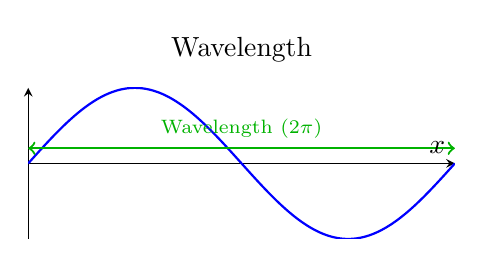
\begin{tikzpicture}
      \begin{axis}[
        axis lines = middle,
        xlabel = $x$,
        xtick=\empty,
        ytick=\empty,
        width=7cm,
        height=3.5cm,
        domain=0:2*pi,
        samples=200,
        title={Wavelength}
      ]
        \addplot[thick, blue] {sin(deg(x))};
        \draw[<->, green!70!black, thick] (axis cs:0,0.2) -- (axis cs:2*pi,0.2) node[midway, above] {\scriptsize Wavelength ($2\pi$)};
      \end{axis}
    \end{tikzpicture}
    \caption{The horizontal distance for one full cycle.}
  \end{subfigure}

  \vspace{0.8cm}

  % Second row: Frequency (left) and Phase (right)
  \begin{subfigure}[t]{0.45\textwidth}
    \centering
    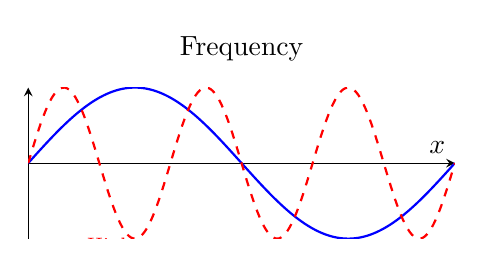
\begin{tikzpicture}
      \begin{axis}[
        axis lines = middle,
        xlabel = $x$,
        xtick=\empty,
        ytick=\empty,
        width=7cm,
        height=3.5cm,
        domain=0:2*pi,
        samples=200,
        title={Frequency}
      ]
        \addplot[thick, blue] {sin(deg(x))};
        \addplot[thick, red, dashed] {sin(deg(3*x))};
        \node[blue] at (axis cs:1.2,1.1) {\scriptsize Low};
        \node[red] at (axis cs:1.2,-1.1) {\scriptsize High};
      \end{axis}
    \end{tikzpicture}
    \caption{More cycles = higher frequency.}
  \end{subfigure}
  \hfill
  \begin{subfigure}[t]{0.45\textwidth}
    \centering
    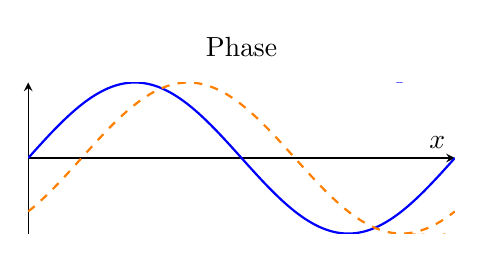
\begin{tikzpicture}
      \begin{axis}[
        axis lines = middle,
        xlabel = $x$,
        xtick=\empty,
        ytick=\empty,
        width=7cm,
        height=3.5cm,
        domain=0:2*pi,
        samples=200,
        title={Phase}
      ]
        \addplot[thick, blue] {sin(deg(x))};
        \addplot[thick, orange, dashed] {sin(deg(x - pi/4))};
        \node[blue] at (axis cs:5.5,1.1) {\scriptsize Original};
        \node[orange] at (axis cs:6.1,-1.1) {\scriptsize Shifted};
      \end{axis}
    \end{tikzpicture}
    \caption{Phase shift moves the wave left or right.}
  \end{subfigure}

  \caption{The four basic properties of waves: amplitude, wavelength, frequency, and phase.}
\end{figure}




To begin, we define the function \textbf{\( u(x, t) \) as \textit{vertical displacement} of a point on the string at position \( x \) and time \( t \)}. In other words, \( u(x, t) \) tells us how much the string is displaced from its equilibrium position at a given location \( x \) and time \( t \). 


\begin{figure}[H]
  \centering
  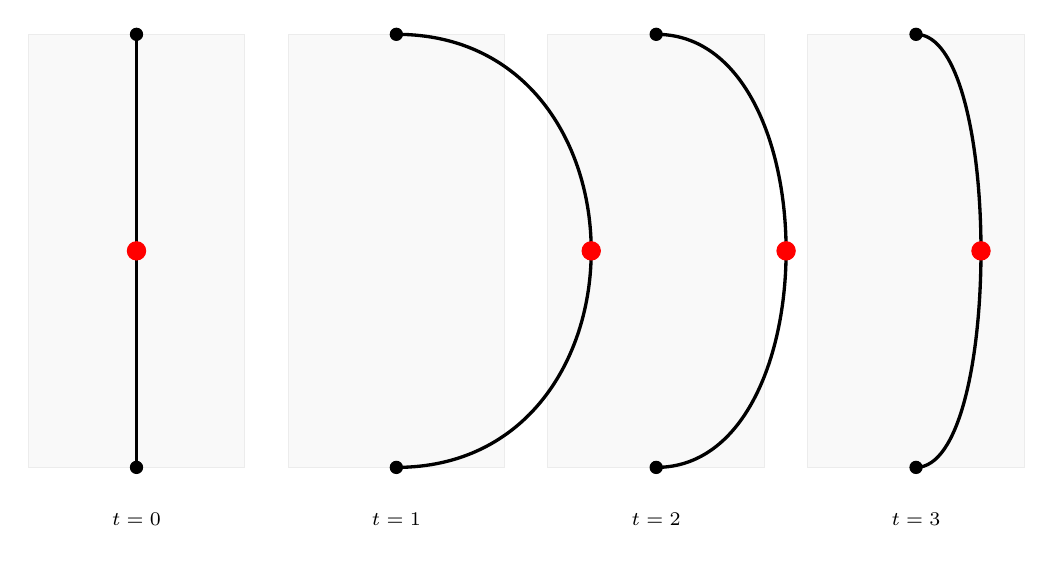
\begin{tikzpicture}[scale=1.1]

    % Constants
    \def\topY{2.5}
    \def\midY{0}
    \def\botY{-2.5}
    \def\panelWidth{2.5}

    % === First Pass: Draw all panel backgrounds and fixed points ===
    \foreach \xshift/\timeLabel in {
      0/0,
      3/1,
      6/2,
      9/3
    } {
      \begin{scope}[xshift=\xshift cm]
        % Background rectangle
        \draw[gray!15, fill=gray!05] (-\panelWidth/2,\botY) rectangle (\panelWidth/2,\topY);

        % Fixed endpoints
        \filldraw[black] (0,\topY) circle (2pt);
        \filldraw[black] (0,\botY) circle (2pt);

        % Time label
        \node at (0,\botY - 0.6) {\scriptsize $t = \timeLabel$};
      \end{scope}
    }

    % === Second Pass: Draw Bézier curves and manually placed red dots ===
    % Format: xshift / control point x / red dot x
    \foreach \xshift/\ctrlX/\redX in {
      0/0/0,
      3/3/2.25,
      6/2/1.5,
      9/1/0.75
    } {
      \begin{scope}[xshift=\xshift cm]
        % Bézier curve
        \draw[very thick] (0,\topY)
          .. controls (\ctrlX,\topY) and (\ctrlX,\botY) ..
          (0,\botY);

        % Manually placed red dot at height = 0
        \filldraw[red] (\redX,\midY) circle (3pt);
      \end{scope}
    }

  \end{tikzpicture}
  \caption{Manual version: each panel shows a vertical string with fixed endpoints (black dots). The Bézier curve shape is controlled via control points, and the red dot is placed manually to show the displacement \( u(x, t) \).}
\end{figure}

\vspace{1.5em}


The displacement changes over time in an oscillating fashion. The motion this vibrating string describes the displacement that varies over both space and time, and the wave equation models how this displacement evolves.

\begin{figure}[H]
\centering
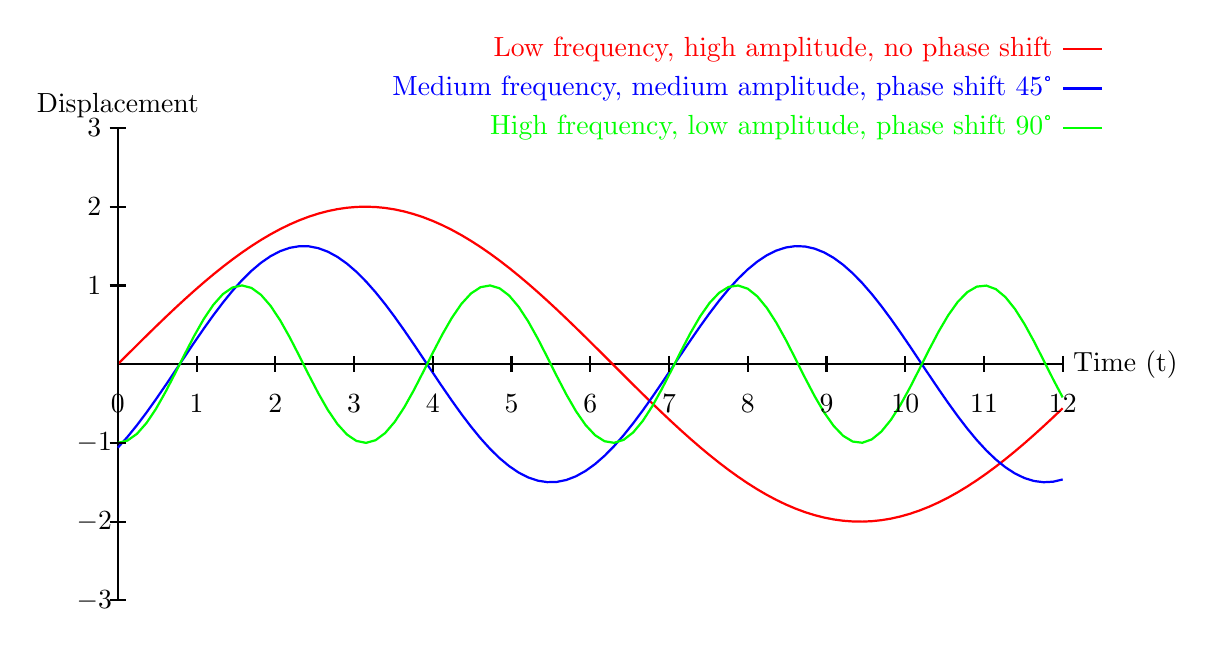
\begin{tikzpicture}

% Draw the x-axis (time axis)
\draw[thick] (0,0) -- (12,0) node[right] {Time (t)};

% Draw the y-axis (displacement axis)
\draw[thick] (0,-3) -- (0,3) node[above] {Displacement};

% Draw waveforms with different frequencies, amplitudes, and wavelengths, with phase shifts

% Wave with low frequency (longer wavelength), no phase shift
\draw[thick, red] plot[domain=0:12,samples=100] (\x,{2*sin(0.5*\x r)}) node[pos=1, above right] {};

% Wave with medium frequency and medium amplitude, with phase shift of 45 degrees
\draw[thick, blue] plot[domain=0:12,samples=100] (\x,{1.5*sin(1*\x r - 45)}) node[pos=1, above right] {};

% Wave with high frequency (shorter wavelength), with phase shift of 90 degrees
\draw[thick, green] plot[domain=0:12,samples=100] (\x,{1*sin(2*\x r - 90)}) node[pos=1, above right] {};

% Adding tick marks for position x on the x-axis (time intervals)
\foreach \x in {0, 1, 2, 3, 4, 5, 6, 7, 8, 9, 10, 11, 12} {
    \draw[shift={(\x,0)}, thick] (0,3pt) -- (0,-3pt);
    \node at (\x,-0.5) {$\x$};
}

% Adding tick marks for position y on the y-axis (displacement)
\foreach \y in {-3,-2,-1,1,2,3} {
    \draw[shift={(0,\y)}, thick] (-3pt,0) -- (3pt,0);
    \node at (-0.3,\y) {$\y$};
}

% Legend for frequency, amplitude, wavelength, and phase shift
\draw[thick, red] (12.5,4) -- (12,4)  node[left] {Low frequency, high amplitude, no phase shift};
\draw[thick, blue]  (12.5,3.5) -- (12,3.5) node[left] {Medium frequency, medium amplitude, phase shift 45°};
\draw[thick, green]  (12.5,3) -- (12,3) node[left] {High frequency, low amplitude, phase shift 90°};

\end{tikzpicture}
\caption{Illustration of different waveforms with varying frequencies, amplitudes, wavelengths, and phase shifts. The red curve represents a wave with low frequency and high amplitude, with no phase shift. The blue curve represents a wave with medium frequency and amplitude, with a phase shift of 45°. The green curve represents a wave with high frequency and low amplitude, with a phase shift of 90°. The legend explains the characteristics of each wave.}
\end{figure}

\vspace{1.5em}


In the context of a vibrating string, these wave properties are not just abstract concepts — they’re fundamental to how the wave behaves and how the PDE is solved.

To get an intuitive feel for this, imagine plucking a taut string like on a guitar. The shape of the wave that travels down the string depends on 

\begin{enumerate}
	\item how hard you pull it \textbf{(amplitude)}, 
	\item how tightly the string is held (which affects \textbf{frequency and wavelength}), 
	\item and exactly where and when you let go (which influences the \textbf{phase}). 
\end{enumerate}
	
The motion that follows can be predicted and described using the wave equation — a mathematical way of capturing that energy rippling back and forth through the string.



\subsection{Smoothing the World: Heat, Harmonics, and the Birth of Fourier Analysis}

Now, let's come back to Fourier's heat equation:

\[
\frac{\partial u}{\partial t} = \alpha \frac{\partial^2 u}{\partial x^2}
\]


This tells us how the temperature \( u(x, t) \) changes over time (\( \frac{\partial u}{\partial t} \)) based on how curved or uneven the temperature is across space (\( \frac{\partial^2 u}{\partial x^2} \)). 

Solving a differential equation means figuring out what the temperature is at every point and time, given how it spreads and smooths out.

\begin{figure}[H]
\centering
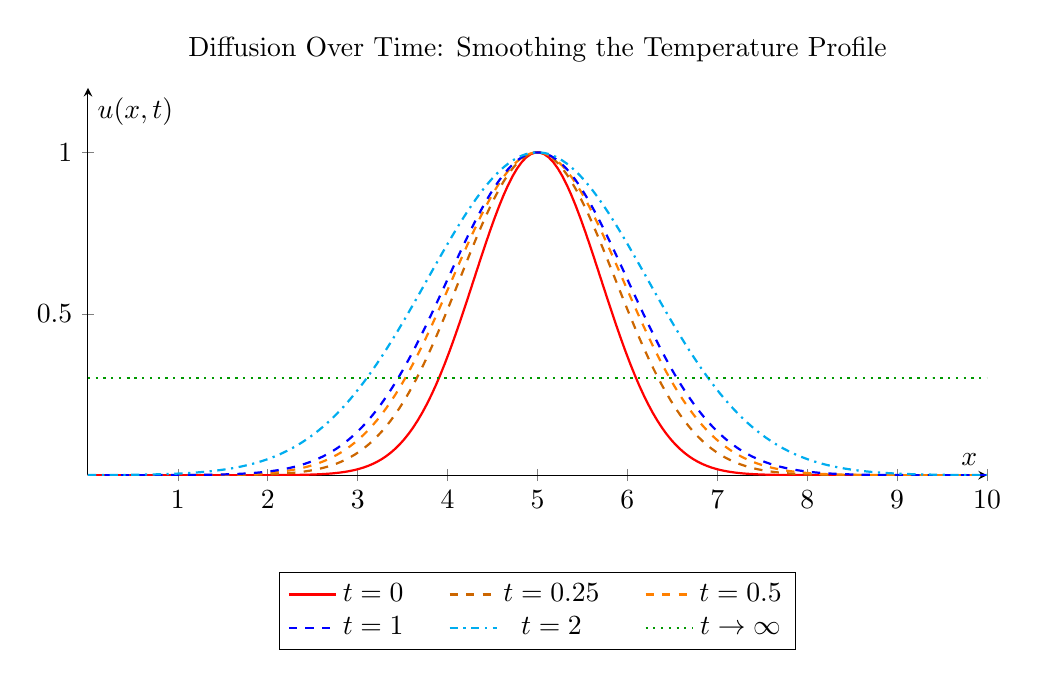
\begin{tikzpicture}
  \begin{axis}[
    domain=0:10,
    samples=200,
    axis lines = middle,
    xlabel = {$x$},
    ylabel = {$u(x, t)$},
    xmin=0, xmax=10,
    ymin=0, ymax=1.2,
    width=13cm,
    height=6.5cm,
    legend style={
      at={(0.5,-0.25)},
      anchor=north,
      legend columns=3,
      /tikz/every even column/.append style={column sep=0.5cm}
    },
    title={Diffusion Over Time: Smoothing the Temperature Profile}
  ]

    % t = 0
    \addplot[thick, red] {exp(-((x-5)^2))};
    \addlegendentry{$t = 0$}

    % t = 0.25
    \addplot[thick, orange!80!black, dashed] {exp(-((x-5)^2)/1.5)};
    \addlegendentry{$t = 0.25$}

    % t = 0.5
    \addplot[thick, orange, dashed] {exp(-((x-5)^2)/1.8)};
    \addlegendentry{$t = 0.5$}

    % t = 1
    \addplot[thick, blue, dashed] {exp(-((x-5)^2)/2)};
    \addlegendentry{$t = 1$}

    % t = 2
    \addplot[thick, cyan, dashdotted] {exp(-((x-5)^2)/3)};
    \addlegendentry{$t = 2$}

    % t → ∞
    \addplot[thick, green!60!black, dotted] {0.3};
    \addlegendentry{$t \rightarrow \infty$}

  \end{axis}
\end{tikzpicture}
\caption{The heat equation smooths out temperature differences over time. An initial sharp spike gradually diffuses and levels into a uniform profile.}
\end{figure}




To solve this kind of differential equation, Fourier looked for functions whose behavior under differentiation was easy to predict. He noticed that sine and cosine functions are especially convenient: when you take their second derivative, you simply get the same function back (up to a negative constant). For example:

\[
\frac{d^2}{dx^2} \sin(nx) = -n^2 \sin(nx)
\]

This property made sines and cosines ideal building blocks for constructing solutions to the heat equation.

\begin{figure}[H]
\centering
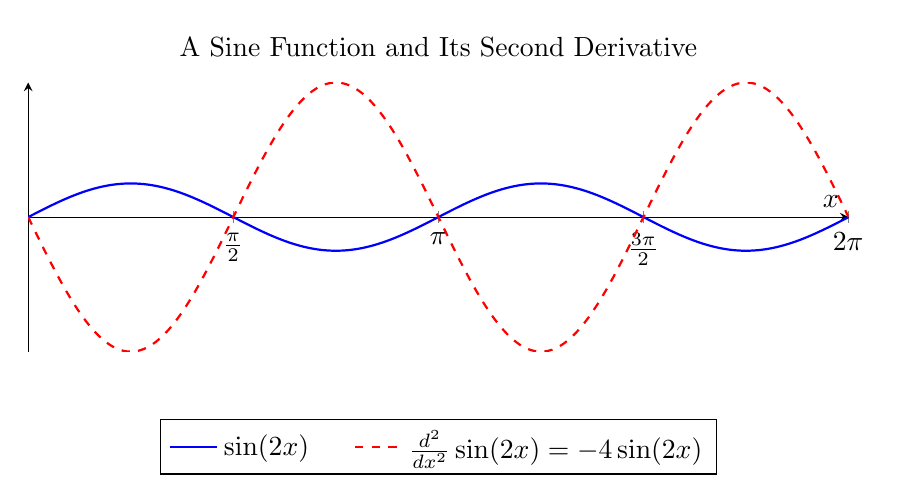
\begin{tikzpicture}
  \begin{axis}[
    domain=0:2*pi,
    samples=200,
    axis lines=middle,
    xlabel={$x$},
    ylabel={},
    xtick={0, 1.57, 3.14, 4.71, 6.28},
    xticklabels={$0$, $\frac{\pi}{2}$, $\pi$, $\frac{3\pi}{2}$, $2\pi$},
    ytick=\empty,
    width=12cm,
    height=5cm,
    legend style={
      at={(0.5,-0.25)},
      anchor=north,
      legend columns=2,
      /tikz/every even column/.append style={column sep=0.5cm}
    },
    title={A Sine Function and Its Second Derivative}
  ]
    % Original sine wave: sin(nx), n=2
    \addplot[thick, blue] {sin(deg(2*x))};
    \addlegendentry{$\sin(2x)$}

    % Second derivative: -n^2 sin(nx) = -4 sin(2x)
    \addplot[thick, red, dashed] {-4*sin(deg(2*x))};
    \addlegendentry{$\frac{d^2}{dx^2} \sin(2x) = -4\sin(2x)$}

  \end{axis}
\end{tikzpicture}
\caption{The second derivative of $\sin(nx)$ is $-n^2 \sin(nx)$ — the same shape, flipped and scaled. This makes sine functions ideal for solving the heat equation.}
\end{figure}



Because of this predictable behavior under differentiation, sines and cosines turn out to be ideal building blocks for solving the heat equation. Using the \textit{separation of variables} method, Fourier could break the problem into parts, each involving one of these wave-like functions. The boundary conditions of physical systems—like a metal rod with its ends held at zero temperature—naturally align with sine and cosine solutions, making them a perfect fit.

A helpful way to understand this is to imagine heat like a drop of ink spreading through water. At first, the ink is concentrated in one spot, but over time, it spreads out smoothly in all directions. The heat equation describes this process mathematically — how temperature (like the ink) diffuses through a material.


Just like you could describe the initial shape of the ink blob using a combination of smooth wave patterns, Fourier realized that any temperature distribution could be broken down into a sum of sine and cosine waves. Each wave evolves over time in a predictable way, and together, they describe how the entire system changes. This is the essence of the Fourier Series applied to heat flow.

\begin{figure}[H]
  \centering

  % First row: Initial and Decomposition
  \begin{subfigure}[t]{0.45\textwidth}
    \centering
    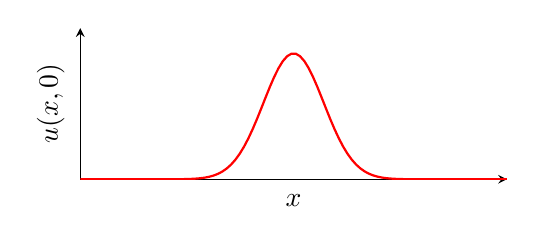
\begin{tikzpicture}
      \begin{axis}[
        axis lines = left,
        xlabel = $x$,
        ylabel = {$u(x, 0)$},
        domain=0:10,
        samples=100,
        ymin=0, ymax=1.2,
        xtick=\empty,
        ytick=\empty,
        width=7cm,
        height=3.5cm,
      ]
        \addplot[thick, red] {exp(-((x-5)^2))};
      \end{axis}
    \end{tikzpicture}
    \caption{Initial heat distribution, concentrated at the center like a drop of ink.}
  \end{subfigure}
  \hfill
  \begin{subfigure}[t]{0.45\textwidth}
    \centering
    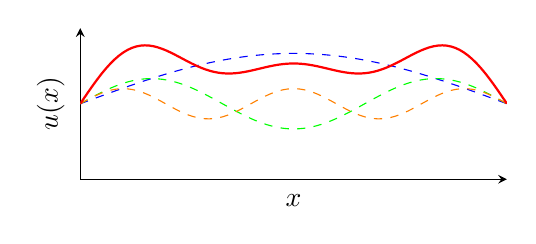
\begin{tikzpicture}
      \begin{axis}[
        axis lines = left,
        xlabel = $x$,
        ylabel = {$u(x)$},
        domain=0:10,
        samples=100,
        ymin=-1.5, ymax=1.5,
        xtick=\empty,
        ytick=\empty,
        width=7cm,
        height=3.5cm,
      ]
        \addplot[blue, dashed] {sin(deg(pi*x/10))};
        \addplot[green, dashed] {0.5*sin(deg(3*pi*x/10))};
        \addplot[orange, dashed] {0.3*sin(deg(5*pi*x/10))};
        \addplot[thick, red] {sin(deg(pi*x/10)) + 0.5*sin(deg(3*pi*x/10)) + 0.3*sin(deg(5*pi*x/10))};
      \end{axis}
    \end{tikzpicture}
    \caption{The initial profile as a sum of sine waves of different frequencies.}
  \end{subfigure}

  \vspace{0.8cm}

  % Second row: Time evolution and final state
  \begin{subfigure}[t]{0.45\textwidth}
    \centering
    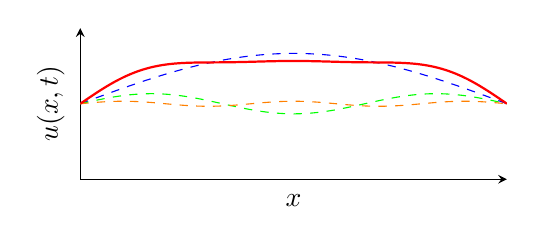
\begin{tikzpicture}
      \begin{axis}[
        axis lines = left,
        xlabel = $x$,
        ylabel = {$u(x, t)$},
        domain=0:10,
        samples=100,
        ymin=-1.5, ymax=1.5,
        xtick=\empty,
        ytick=\empty,
        width=7cm,
        height=3.5cm,
      ]
        \addplot[blue, dashed] {sin(deg(pi*x/10))};
        \addplot[green, dashed] {0.2*sin(deg(3*pi*x/10))};
        \addplot[orange, dashed] {0.05*sin(deg(5*pi*x/10))};
        \addplot[thick, red] {sin(deg(pi*x/10)) + 0.2*sin(deg(3*pi*x/10)) + 0.05*sin(deg(5*pi*x/10))};
      \end{axis}
    \end{tikzpicture}
    \caption{Over time, high-frequency components decay faster.}
  \end{subfigure}
  \hfill
  \begin{subfigure}[t]{0.45\textwidth}
    \centering
    \begin{tikzpicture}
      \begin{axis}[
        axis lines = left,
        xlabel = $x$,
        ylabel = {$u(x, t \to \infty)$},
        domain=0:10,
        samples=2,
        ymin=0, ymax=1.2,
        xtick=\empty,
        ytick=\empty,
        width=7cm,
        height=3.5cm,
      ]
        \addplot[thick, blue] coordinates {(0,0.4) (10,0.4)};
      \end{axis}
    \end{tikzpicture}
    \caption{Eventually, the temperature becomes uniform.}
  \end{subfigure}

  \caption{Fourier analysis of heat flow: from initial condition to spectral decomposition and smoothing over time.}
\end{figure}


He understood that sine and cosine functions possess a special property called orthogonality. In simple terms, this means that when you compare different sine and cosine waves over a complete cycle — say, by calculating how much they "overlap" through integration — their contributions to each other cancel out perfectly. They’re like two dancers moving in rhythm but on completely different paths: one moves side-to-side, the other up-and-down, and no matter how long you watch them, their motions never reinforce or interfere with each other.

Mathematically, this orthogonality means that if you multiply, for example, a sine wave and a cosine wave of the same frequency and integrate the result over a full period (like one full oscillation), you get zero. It’s as if one wave is completely “invisible” to the other when measuring energy or contribution across time.

You can think of this like tuning forks that vibrate at different frequencies — strike one, and the others don’t resonate unless they’re tuned the same way. Or imagine shining red and green lights onto a screen: their colors don’t mix unless you explicitly combine them. Similarly, in the Fourier series, each sine and cosine function only captures its own frequency component — it ignores everything else. That’s what makes them such a powerful basis for building up complicated waveforms: each part contributes cleanly and independently, without muddying the signal.

This insight is what allows Fourier series to break down any periodic function into a clean sum of sinusoids — each part precisely measures just one "ingredient" in the recipe, with no cross-talk between them.

\begin{figure}[H]
    \centering
    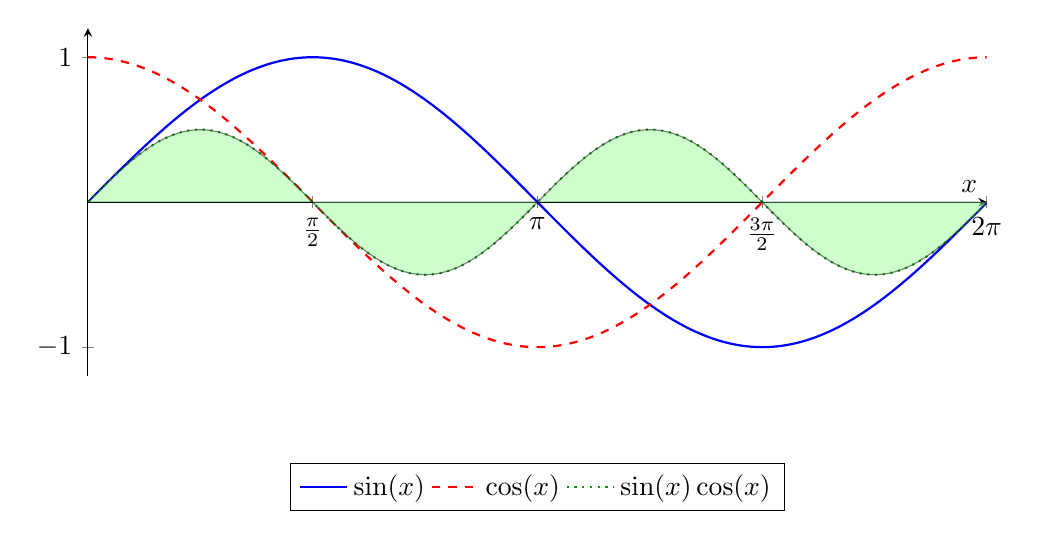
\begin{tikzpicture}
        \begin{axis}[
            width=13cm,
            height=6cm,
            axis lines=middle,
            xlabel={$x$},
            ylabel={},
            xtick={0, 1.57, 3.14, 4.71, 6.28},
            xticklabels={$0$, $\frac{\pi}{2}$, $\pi$, $\frac{3\pi}{2}$, $2\pi$},
            ytick={-1,0,1},
            ymin=-1.2, ymax=1.2,
            samples=300,
            domain=0:6.28,
            legend style={at={(0.5,-0.25)}, anchor=north, legend columns=3},
            clip=true,
        ]
            % sin(x)
            \addplot [blue, thick] {sin(deg(x))};
            % cos(x)
            \addplot [red, thick, dashed] {cos(deg(x))};
            % sin(x)cos(x)
            \addplot [green!60!black, thick, dotted] {sin(deg(x))*cos(deg(x))};

            % Fill positive area
            \addplot [
                domain=0:pi,
                fill=green!40,
                opacity=0.5,
            ] {sin(deg(x))*cos(deg(x))} \closedcycle;

            % Fill negative area
            \addplot [
                domain=pi:2*pi,
                fill=green!40,
                opacity=0.5,
            ] {sin(deg(x))*cos(deg(x))} \closedcycle;

            \legend{$\sin(x)$, $\cos(x)$, $\sin(x)\cos(x)$}
        \end{axis}
    \end{tikzpicture}
    \caption{Orthogonality of $\sin(x)$ and $\cos(x)$: The product $\sin(x)\cos(x)$ has symmetric positive and negative areas over $[0, 2\pi]$, which cancel out when integrated.}
    \label{fig:sin_cos_cancellation}
\end{figure}


\subsection{From Equations to Oscillations}

In Jacobi’s mechanics, every trajectory was a path across a surface;  
in Cayley’s algebra, every transformation was a matrix;  
in Fourier’s world, every motion—no matter how irregular—was a sum of oscillations.

Motion was no longer a path to be solved;  
it was a frequency spectrum to be unpacked.

In studying heat flow, Fourier discovered that even the most tangled temperature distributions could be written as a sum of simple waves—  
waves that added, canceled, and recombined to produce the observed pattern.

The insight ran deeper than heat:  
vibrations of strings, the motion of celestial bodies, the sound of instruments, even solutions to partial differential equations—  
all could be analyzed by projecting them onto a basis of sinusoidal functions.

\subsection{From Structure to Frequency}

Cayley had abstracted geometry into algebraic operations;  
Fourier abstracted function behavior into frequency content.

Where Cayley studied invariance under transformations of space,  
Fourier studied invariance under transformations of representation:  
switching from position to frequency, from time to spectrum.

This was more than a computational trick; it was a conceptual inversion:

\begin{itemize}
  \item Instead of describing a system in terms of where it is,  
  \item describe it in terms of \textbf{how it vibrates.}
\end{itemize}


\begin{quote}
In Euler, we computed forces.  
In Lagrange, we minimized action.  
In Hamilton, we traced flows.  
In Jacobi, we found surfaces.  
In Cayley, we abstracted transformations.  
In Fourier, we decomposed everything into vibration.
\end{quote}

\subsection{The Geometry Hidden in Waves}

Fourier’s decomposition hinted at a deeper structure:  
that even the most complex behaviors might arise from the linear combination of simple modes.

Later mathematicians would realize that this decomposition was tied to eigenvalues and eigenvectors of operators—  
connecting Fourier’s analysis back to Cayley’s matrices, and forward into Hilbert spaces and functional analysis.

And just as Cayley turned geometry into algebra,  
Fourier turned analysis into geometry of function spaces,  
where each function was a point, and each frequency component an axis.

The door was now open for a new synthesis:  
where geometry, algebra, and analysis converged into the language of inner products, linear operators, and spectral theory.

And it would be in this convergence that the mathematics of waves, mechanics, and geometry would find a new home—  
a home that Riemann, Hilbert, and Einstein would soon inhabit.


\subsection{Reinterpreting Kepler’s Second Law Through Fourier’s Lens}

Kepler’s Second Law tells us that a planet sweeps out equal areas in equal times—  
a principle that speaks of symmetry, conservation, and geometric regularity.

But what if this law, like all others in mechanics, could be reframed in the language of vibration?

\bigskip

\begin{tcolorbox}[colback=purple!5!white, colframe=purple!80!black, title=\textbf{Fourier's View: Kepler as Spectral Balance}]
Planetary motion is not just a path through space—  
it is a \textbf{superposition of orbital modes},  
and Kepler’s Second Law encodes the conservation of angular frequency content over time.
\end{tcolorbox}

\bigskip

\paragraph{From Area to Oscillation.}

In Hamiltonian mechanics, Kepler’s Second Law arises from conservation of angular momentum.  
But in Fourier’s framework, angular momentum corresponds to a \textbf{dominant frequency mode}—  
a persistent component in the system’s motion that remains constant over time.

That is:

\begin{itemize}
  \item The angular sweep of a planet becomes a periodic signal,
  \item Its velocity vector traces out a time-varying waveform,
  \item And the constancy of swept area becomes the \textbf{invariance of the lowest-frequency term} in the planet’s angular dynamics.
\end{itemize}

\bigskip

\paragraph{Orbital Motion as Harmonic Content.}

Keplerian ellipses are not random curves; they are highly structured,  
and their motion can be projected onto a Fourier basis in time:

\[
\theta(t) \approx \sum_{n} A_n \sin(n\omega t + \phi_n)
\]

In this view, the planet’s areal velocity corresponds to the preservation of a fundamental mode \( \omega \)—  
a rotation frequency around the central body.

Equal areas in equal times becomes a constraint on how that frequency content can evolve:  
the spectral energy of the motion must remain concentrated in the same harmonic band.

\bigskip

\paragraph{Spectral Conservation.}

Where Jacobi saw surfaces and Cayley saw transformations,  
Fourier saw oscillations whose amplitudes and phases tell the full story of the orbit.

Kepler’s Second Law is thus recast as a constraint in the frequency domain:  
a law of motion that conserves not just a geometric quantity,  
but the \textbf{spectrum of motion itself}.

\bigskip

\begin{quote}
Kepler measured sweep.\\
Hamilton measured flux.\\
Fourier measured frequency.\\
And the law endured in every representation.
\end{quote}